\documentclass[a4paper, 12pt, titlepage]{article}
\usepackage[utf8]{inputenc}
\usepackage{geometry}
\usepackage{polski}
\usepackage{graphicx}
\usepackage{float}
\usepackage{etoolbox,refcount}
\usepackage{multicol}

\title{Badanie właściwości metrologicznych toru pomiarowego z modulacją AM przeznaczonego do współpracy z czujnikami wielkości nieelektrycznych}
\author{\textbf{Adrian Jałoszewski}, Tomasz Kotowski, Monika Ścisło}
\date{10 października 2016, poniedziałek, $9^{\underline{30}}$}

\begin{document}
	\maketitle
	\section{Cel ćwiczenia}
	Celem ćwiczenia było zapoznanie się z pomiarem wielkości nieelektrycznej jaką jest przesunięcie przy pomocy przyrządów mierzących wielkości elektryczne.
	\section{Układ}
	
	\begin{figure}[H]
		\centering
		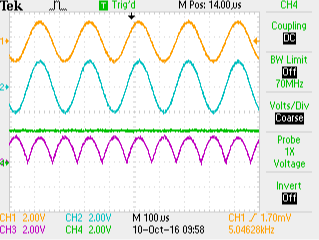
\includegraphics[height=6cm, width=\textwidth]{./img/rozciagniete.png}
	\end{figure}
	
\end{document}